\documentclass[11pt,twocolumn]{article}
\usepackage[left=1in,top=1in,right=1in,bottom=1in,nohead,foot=1cm]{geometry} 
\usepackage{aaai}
\usepackage{times}
\usepackage{tikz}
\usepackage{pgfplots}
\usepackage{amsmath,amssymb}
\usepackage{graphicx,psfrag}
\usepackage{amsthm} 
\usepackage{setspace}
\DeclareMathSymbol{\R}{\mathbin}{AMSb}{"52}

%\doublespacing

\newtheorem{lemma}{Lemma}
\newtheorem{theorem}{Theorem}

\title{GiftGiver: The Gift Recommender \\ {\small AAI --
    Instructor: Prof. Jane Hsu}}
\author{Weiti Kuo, Penn Su, George Chang \\ \{r99922003, r99922157, r99944002\}@csie.ntu.edu.tw}
\begin{document}
\maketitle

\section{Introduction}

Explain the problem and its motivation (why it is important including possible
applications).

\section{Background and Related Work}

Briefly explain relevant work.

\subsection{Specific Papers}
Here, list the 3-4 papers you will focus on, along with a brief intro
that ties them together.


\section{Paper 1 -- An Explanatory Title}
\subsection{Problem Description}
The specific problem addressed in the paper.

\subsection{Preliminaries}
Background material one needs to know to understand this paper
(examples could be support vector machines, markov decision processes,
visibility graphs etc.) along with brief explanations.


\subsection{Approach}
How does the paper solve the problem?

\subsection{Critique}
Pros and cons. Do they make unreasonable assumptions? How do they show
the utility of their results? Do they prove them or provide extensive simulations?


\section{AAI Project}
\subsection{Problem Description}

\subsection{Preliminaries}

\subsection{Approach}

\subsection{Critique}


\section{Evaluation}
It is rather hard to evaluate recommender system, and even so with common sense knowledge because there is no
common criterions to evaluate common sense. However, since we haven't found the state of the art recommender engine
using common sense for gift recommendation, we have conducted a couple surveys and user studies to evaluate the accuracy
of our recommender system.

Based on time constraints, we conducted a usability test and two surveys with five National Taiwan University graduate students and alumnae.
The results of the surveys and the usability test are listed below.

\begin{table*}[ht]
\caption{Usability test results}
\centering
\begin{tabular}{| p{5cm} | c | c | c | c | c |}
\hline
Question & Subject 1 & Subject 2 & Subject 3 & Subject 4 & Subject 5 \\
\hline
Was the UI easy to use? & 3 & 4 & 3 & 3 & 4 \\
\hline
Did the options cover all my considerations for gift recommendation? & 3 & 4 & 3 & 4 & 3 \\
\hline
Were the ideal gifts in the result list? & 4 & 4 & 3 & 4 & 4 \\
\hline
Were most of the recommendations realistic? & 5 & 3 & 3 & 5 & 4 \\
\hline
Was the price checking feature helpful? & 4 & 5 & 5 & 5 & 4 \\
\hline
Will you consider using our system for gift recommendation in the future? & 5 & 4 & 4 & 5 & 4 \\
\hline
\end{tabular}
\label{table:usetest}
\end{table*}

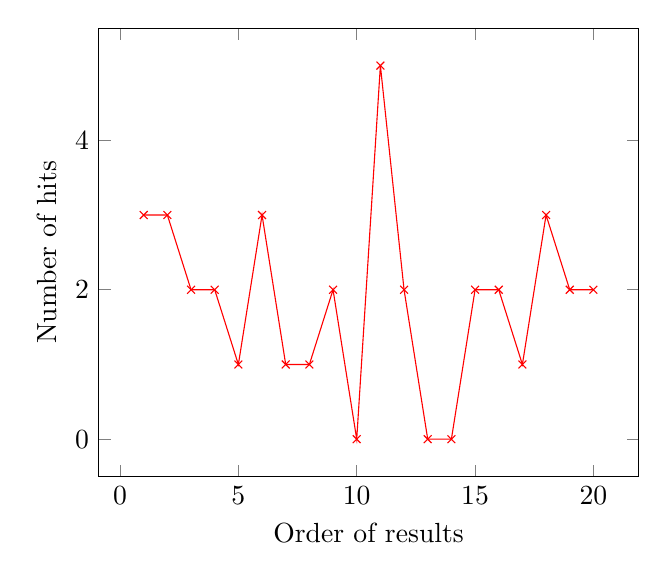
\begin{tikzpicture}
    \begin{axis}[xlabel=Order of results, ylabel=Number of hits]
    \addplot[color=red,mark=x] coordinates {(1,3) (2,3) (3,2) (4,2) (5,1) (6,3) (7,1) (8,1) (9,2) (10,0) (11,5) (12,2) (13,0) (14,0) (15,2) (16,2) (17,1) (18,3) (19,2) (20,2)};
    \end{axis}
\end{tikzpicture}

According to the plot above, the distribution is pretty even through out the search results but some bumpy hills along. We define hit rate as the number of times the tester's desired gift is ``hit'' on the result list. The higher the number the better our system performs. To illustrate the result of our survey in terms of hit rate, the scatter plot below provides the representation for that.

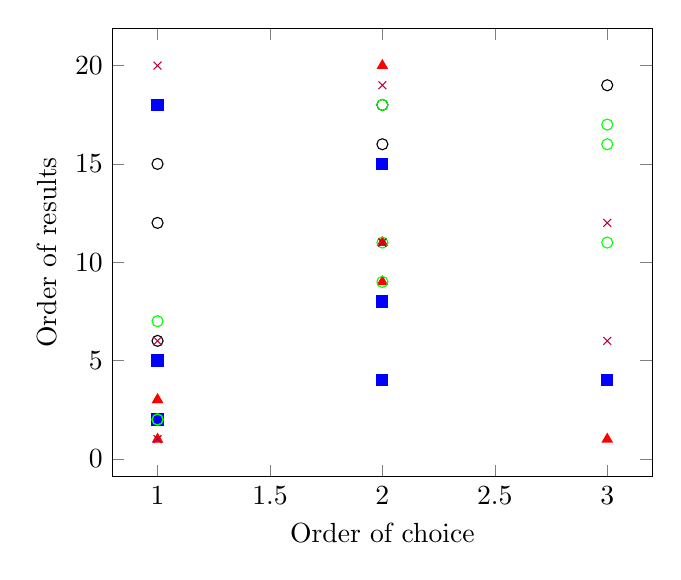
\begin{tikzpicture}
    \begin{axis}[
    xlabel=Order of choice,
    ylabel=Order of results,
    scatter/classes={
    a={mark=square*,blue},%
    b={mark=triangle*,red},%
    c={mark=o,draw=black},
    d={mark=o,draw=green},
    e={mark=x,draw=purple}
    }]
    \addplot[scatter,only marks,scatter src=explicit symbolic] 
    coordinates {
    (1, 5) [a]
    (2, 15) [a]
    (1, 18) [a]
    (2, 8) [a]
    (3, 4) [a]
    (1, 2) [a]
    (2, 4) [a]

    (1, 3) [b]
    (2, 20) [b]
    (1, 1) [b]
    (2, 9) [b]
    (1, 3) [b]
    (2, 11) [b]
    (3, 1) [b]

    (1, 15) [c]
    (1, 6) [c]
    (2, 18) [c]
    (3, 19) [c]
    (1, 12) [c]
    (2, 16) [c]

    (1, 7) [d]
    (2, 18) [d]
    (3, 16) [d]
    (1, 2) [d]
    (2, 11) [d]
    (3, 17) [d]
    (1, 2) [d]
    (2, 9) [d]
    (3, 11) [d]

    (1, 6) [e]
    (2, 11) [e]
    (3, 12) [e]
    (1, 1) [e]
    (2, 11) [e]
    (1, 20) [e]
    (2, 19) [e]
    (3, 6) [e]
    };
    \end{axis}
\end{tikzpicture}


\section{Conclusion}

A comparison of the approaches and contributions of the paper.
What is solved, what is left out.

\bibliography{aai2011}
\bibliographystyle{abbrv}



\end{document}
